\documentclass{article}

%usepackages
\usepackage[margin=0.5in]{geometry}
\usepackage[utf8]{inputenc}
\usepackage{textcomp}
\usepackage{amssymb}

%plots
\usepackage{pgfplots}

%for the table
\usepackage{multirow}
\usepackage{longtable}
\usepackage{array}
\usepackage{booktabs, tabularx}
\usepackage{caption}
\captionsetup[table]{position=above, belowskip=4pt}
\usepackage{ragged2e}

\usepackage{multicol}
\usepackage{blindtext}

\usetikzlibrary{pgfplots.groupplots}
\pgfplotsset{width=15cm,compat=1.9} %size for bigger plot

\begin{document}

	%OnlyPlot
\begin{tikzpicture}
\begin{axis}[
    title={Metallfadenlampe},
    xlabel={Spannung [V]},
    ylabel={Ladung [A]},
    xmin=0, xmax=200,
    ymin=0, ymax=0.4,
    xtick={0,20,40,60,80,100,120,140,160,180,200},
    ytick={0, 0.1, 0.2, 0.3, 0.4},
    legend pos=north west,
    ymajorgrids=true,
    grid style=dashed,
]

\addplot[
    color=blue,
    mark=square,
    ]
    coordinates {
    (0,0)(4,0.006)(14,0.1)(24,0.12)(32,0.13)(41,0.15)(50,0.17)(59,0.19)(68,0.2)(76,0.22)(85,0.23)(93,0.23)(102,0.25)(112,0.26)(120,0.27)(129,0.28)(138,0.3)(147,0.31)(156,0.32)(165,0.33)(174,0.34)(183,0.35)(192,0.35)
    };
    \legend{Wiederstand [$\Omega$]}
    
\end{axis}


\end{tikzpicture}

%================================================================================
			%three Plots
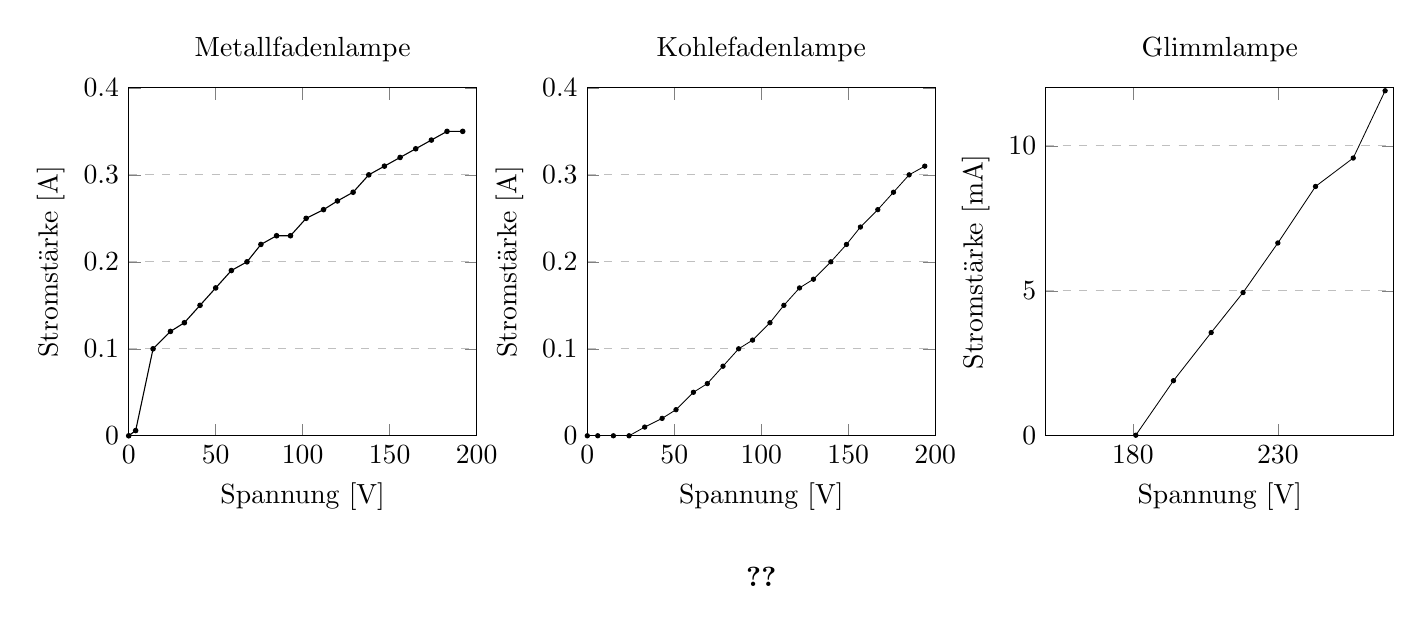
\begin{tikzpicture} 

%Options for every plot but can be overwriten on \nextgroupplot
\begin{groupplot}
[
enlargelimits=0,
legend columns=5,
ymajorgrids=true, 		%activates lines on the plots
grid style=dashed, 		%makes the lines dashed
width=6cm, 		%width of the plots
height=6cm, 		%height of the plots
%xtick={0,50,100,150,200},		 %marks on the x-axe is also genarated
nodes near coords align={vertical},
group style={
group size=3 by 1, %how many plots times plot
xlabels at=edge bottom,
ylabels at=edge left, 
horizontal sep=40pt, %distance betwen plots
xticklabels at=edge bottom}
]
\pgfplotsset{group/every plot/.style={xmin=1,xmax=10}}

%Metallfadenlampe
%Options for the single plots
\nextgroupplot[title={ Metallfadenlampe},
ymin=0, ymax=0.4,xmin=0,xmax=200, 
xlabel={Spannung [V]}, ylabel={Stromstärke [A]},
legend style = { column sep = 10pt, legend columns = -1, legend to name = grouplegend}]
%Options for the Graph
\addplot
[
line width=0.4pt,
color=black,
mark=*,
mark options={scale=0.4}
]
coordinates{
     (0,0)(4,0.006)(14,0.1)(24,0.12)(32,0.13)(41,0.15)(50,0.17)(59,0.19)(68,0.2)(76,0.22)(85,0.23)(93,0.23)(102,0.25)(112,0.26)(120,0.27)(129,0.28)(138,0.3)(147,0.31)(156,0.32)(165,0.33)(174,0.34)(183,0.35)(192,0.35)};
\addlegendentry{$Wiederstand$ $[\Omega]$}

%Kohlefadenlampe
\nextgroupplot[title={ Kohlefadenlampe},
ymin=0, ymax=0.4,xmin=0,xmax=200,
xlabel={Spannung [V]}, ylabel={Stromstärke [A]},
]
\addplot
[
line width=0.3pt,
color=black,
mark=*,
mark options={scale=0.4}
]
coordinates{
   (0,0)(6,0)(15,0)(24,0)(33,0.01)(43,0.02)(51,0.03)(61,0.05)(69,0.06)
   (78,0.08)(87,0.1)(95,0.11)(105,0.13)(113,0.15)(122,0.17)(130,0.18)(140,0.2)(149,0.22)(157,0.24)(167,0.26)(176,0.28)(185,0.3)(194,0.31)};


%Glimmlampe
\nextgroupplot[title={ Glimmlampe},ymin=0, ymax=12,xmin=150,xmax=270, xlabel={Spannung [V]}, ylabel={Stromstärke [mA]},
xtick={180,230,280}]
\addplot
[
line width=0.3pt,
color=black,
mark=*,
mark options={scale=0.4}
]
coordinates{
    (181,0.02)(194,1.9)(207,3.56)(218,4.94)(230,6.65)(243,8.6)(256,9.58)(267,11.9)};


\end{groupplot}
\node at ($(group c2r1) + (0,-4cm)$) {\ref{grouplegend}};
\end{tikzpicture}

\newpage

%============================================================================

%table
\begin{multicols}{3}
%Metallfadelampe
\begin{tabular}{| >{\centering\arraybackslash}m{0.5in} | 
				>{\centering\arraybackslash}m{0.5in} |}
\hline
 \multicolumn{2}{|c|}{Metallfadenlampe}\\
	\hline 
	U[V]	&	I [mA]\\
	\hline
	0	&	0\\
	\hline
	4	&	60\\
	\hline
	14	&	100\\
	\hline
	24	&	120\\
	\hline
	32	&	130\\
	\hline
	41	&	150\\
	\hline
	50	&	170\\
	\hline
	59	&	190\\
	\hline
	68	&	200\\
	\hline
	76	&	220\\
	\hline
	85	&	230\\
	\hline
	93	&	230\\
	\hline
	102	&	250\\
	\hline
	112	&	260\\
	\hline
	120	&	270\\
	\hline
	129	&	280\\
	\hline
	138	&	300\\
	\hline
	147	&	310\\
	\hline
	156	&	320\\
	\hline
	165	&	330\\
	\hline
	174	&	340\\
	\hline
	183	&	350\\
	\hline
	192	&	350\\
	\hline	

\end{tabular}

%Kohlenfadenlampe
\begin{tabular}{| >{\centering\arraybackslash}m{0.5in} 
				|>{\centering\arraybackslash}m{0.5in} |}
\hline
 \multicolumn{2}{|c|}{Kohlenfadenlampe}\\
	\hline 
	U[V]	&	I [mA]\\
	\hline
	0	&	0\\
	\hline
	6	&	0\\
	\hline
	15	&	0\\
	\hline
	24	&	0\\
	\hline
	33	&	10\\
	\hline
	43	&	20\\
	\hline
	51	&	30\\
	\hline
	61	&	50\\
	\hline
	69	&	60\\
	\hline
	78	&	80\\
	\hline	
	87	&	100\\
	\hline
	95	&	110\\
	\hline
	105	&	130\\
	\hline
	113	&	150\\
	\hline
	122	&	170\\
	\hline
	130	&	180\\
	\hline
	140	&	200\\
	\hline	
	149	&	220\\
	\hline
	157	&	240\\
	\hline
	167	&	260\\
	\hline
	176	&	280\\
	\hline
	185	&	300\\
	\hline
	194	&	310\\
	\hline	
\end{tabular}

%Glimmlampe
\begin{tabular}{|c|c|}
\hline
 \multicolumn{2}{|c|}{Glimmlampe}\\
	\hline 
	U[V]	&	I [mA]\\
	\hline
	181	&	0.02\\
	\hline
	194	&	1.9\\
	\hline
	207	&	3.56\\
	\hline
	218	&	4.94\\
	\hline
	230	&	6.65\\
	\hline
	243	&	8.6\\
	\hline
	256	&	9.58\\
	\hline
	267	&	11.9\\
	\hline

\end{tabular}

\end{multicols}
\pagebreak

%=============================================================================
 
 \begin{center}
\begin{tabular}{ |c|c|c|c| } 
\hline
 \multicolumn{4}{|c|}{Country List} \\
 \hline
col1 & col2 & col3  & col4\\
\hline
\multirow{4}{4em}{Multiple row} 
& cell2 & cell3 & cell10\\ 
& cell5 & cell6 &cell11\\ 
& cell8 & cell9 & cell12\\ 
\hline
\end{tabular}
\end{center}

\begin{tabular}{ |p{3cm}||p{3cm}|p{3cm}|p{3cm}|  }
 \hline
 \multicolumn{4}{|c|}{Country List} \\
 \hline
 Country Name     or Area Name& ISO ALPHA 2 Code &ISO ALPHA 3 Code&ISO numeric Code\\
 \hline
 Afghanistan   & AF    &AFG&   004\\
 Aland Islands&   AX  & ALA   &248\\
 Albania &AL & ALB&  008\\
 Algeria    &DZ & DZA&  012\\
 American Samoa&   AS  & ASM&016\\
 Andorra& AD  & AND   &020\\
 Angola& AO  & AGO&024\\
 \hline
\end{tabular}

 \begin{longtable}[c]{| c | c |}
 \caption{Long table caption.\label{long}}\\

 \hline
 \multicolumn{2}{| c |}{Begin of Table}\\
 \hline
 Something & something else\\
 \hline
 \endfirsthead

 \hline
 \multicolumn{2}{|c|}{Continuation of Table \ref{long}}\\
 \hline
 Something & something else\\
 \hline
 \endhead

 \hline
 \endfoot

 \hline
 \multicolumn{2}{| c |}{End of Table}\\
 \hline\hline
 \endlastfoot

 Lots of lines & like this\\
 Lots of lines & like this\\
 Lots of lines & like this\\
 Lots of lines & like this\\
 Lots of lines & like this\\
 Lots of lines & like this\\
 Lots of lines & like this\\
 Lots of lines & like this\\
 ...
 Lots of lines & like this\\
 \end{longtable}

\begin{multicols}{2}
\begin{tabular}{|c|c|}
el&el2\\
\hline
el3&el4\\
\hline
\end{tabular}


\begin{tabular}{|c|c|}
el&el2\\
\hline
el3&el4\\
\hline
\end{tabular}

\end{multicols}




\begin{table}
\parbox{.45\linewidth}{
\centering
\begin{tabular}{|c|c|}

\hline
a&b\\
\hline
\end{tabular}
\caption{Foo}
}
\hfill
\parbox{.45\linewidth}{
\centering
\begin{tabular}{|c|c|}
\hline
d&e\\
\hline
\end{tabular}
\caption{Bar}
}
\end{table}






\begin{table}[htbp]
\caption{filter window size}
\label{tab:config_filternum}
 \begin{tabularx}{.5\textwidth}{| X | X | c |} 
 \hline
 number of entity filter (size 1) & number of context filters (size 2, size 3,
 size 4) & Accuracy\\ [2ex] 
 \hline
    32  &  32  ,  32  ,  32  &  0.835 \\ [0.5ex]
    \hline
    32  &  64  ,  64  ,  64  &  0.821 \\ [0.5ex]
    \hline
    \hline
 \end{tabularx}
 \quad
\begin{tabularx}{.5\textwidth}{| X | X | c |} 
 \hline
 number of entity filter (size 1) & number of context filters (size 2, size 3,
 size 4) & Accuracy\\ [2ex] 
 \hline
512  &  32  ,  32  ,  32  &  0.910 \\[0.5ex]
\hline
512  &  64  ,  64  ,  64  &  0.922 \\[0.5ex]
\hline
\hline
\end{tabularx}
\end{table}

%=============================================================================





\end{document}
